\chapter{Implementierung des MRCPSP-Frameworks} \label{ch:Implementierung}
In diesem Kapitel wird die Implementierung des \ac{mrcpsp}-Frameworks einschließlich der entwickelten Metaheuristiken vorgestellt. Zunächst gilt es die Struktur des Frameworks im Abschnitt \ref{sec:Strukturbeschreibung} basierend auf einem UML-Klassendiagramm aufzuzeigen. Das Thema der Zeitplanerstellung, Heuristiken und die Visualisierung wird im Folgeabschnitt behandelt. Abschnitt \ref{sec:Loesungsansaetze} stellt die unterschiedlich implementierten Lösungsansätze und Metaheuristiken vor. Der Aufbau von Experimenten, wie beispielsweise der Vergleich von den Lösungsansätzen oder die Handhabung von Unsicherheitsszenarien gilt es im Abschnitt \ref{sec:Experimente} zu vertiefen. % Zuletzt wird die Umsetzung von Visualisierungen im Abschnitt \ref{sec:Visualisierung} behandelt. 

\section{Strukturbeschreibung} \label{sec:Strukturbeschreibung}

Wie bereits im Abschnitt \ref{sec:Konzeptüberblick} erläutert wird für die Entwicklung des MRCPSP Framework die objektorientierte Programmiersprache Java einschließlich des Spring genutzt. Über die objektorientierte Programmierung können Teilaspekte der Anwendung über Klassen voneinander getrennt werden. Packages können zudem eingesetzt, um Aspekte voneinander zu trennen, um so den Code übersichtlicher zu halten. Innerhalb des MRCPSP Frameworks sind die Packages nach Kategorien angelegt. Folgende Paketstruktur ist mit entsprechenden Funktionen in der Umsetzung vorgesehen:

\begin{description}
\item[Rootpackage] \lstinline|de.uol.sao.rcpsp_framework| beinhaltet die Mainklasse und somit den Einstiegspunkt der Anwendung. Durch die Verwendung vom Spring Framework werden weitere Einstiegspunkte in der Anwendung über die Komponenten/Services Annotation festgelegt. 
\item[exception] Eigene Exceptions die innerhalb der Anwendung auftreten sind in diesem Package enthalten.
\item[experiment] Einzelne zu untersuchende Aspekte werden über Experimente geregelt.  
\item[heuristic] Klassen zur Generierung von Aktivitäts- und Moduslisten anhand bestimmter Prioritäts- und Modusregeln. 
\item[metric] Unterschiedliche Funktionen für Zeitplan-Metriken, um bestimmte Informationen, wie die Projektdauer oder Robustheit zu berechnen. 
\item[function] Zielfunktionen, die entweder für einen direkten Vergleich zweier Zeitpläne oder für die Fitness-Berechnung eines einzelnen Plans eingesetzt werden. 
\item[representation] Unterschiedliche Representationsformen von Aktivitäts- und Modusselektionen für Zeitpläne die innerhalb des \ac{mrcpsp} Frameworks verwendet werden können.
\item[scheduling] Klassen zum Erstellen von Zeitplänen und deren Informationen. 
\item[service] Mit \lstinline{@Service} annotierte Klassen, welche in der kompletten Anwendung an unterschiedlichen Stellen verwendet werden. 
\item[solver] Beliebige Lösungsverfahren u. a. Metaheuristiken, die in der Anwendung verwendet werden.
\item[helper] Hilfsklassen und deren Methoden, die über die komplette Anwendung genutzt werden und sich nicht in anderen Packages klassifizieren lassen. 

\end{description}

\begin{figure}
    \centering
    \noindent\makebox[\textwidth]{%
    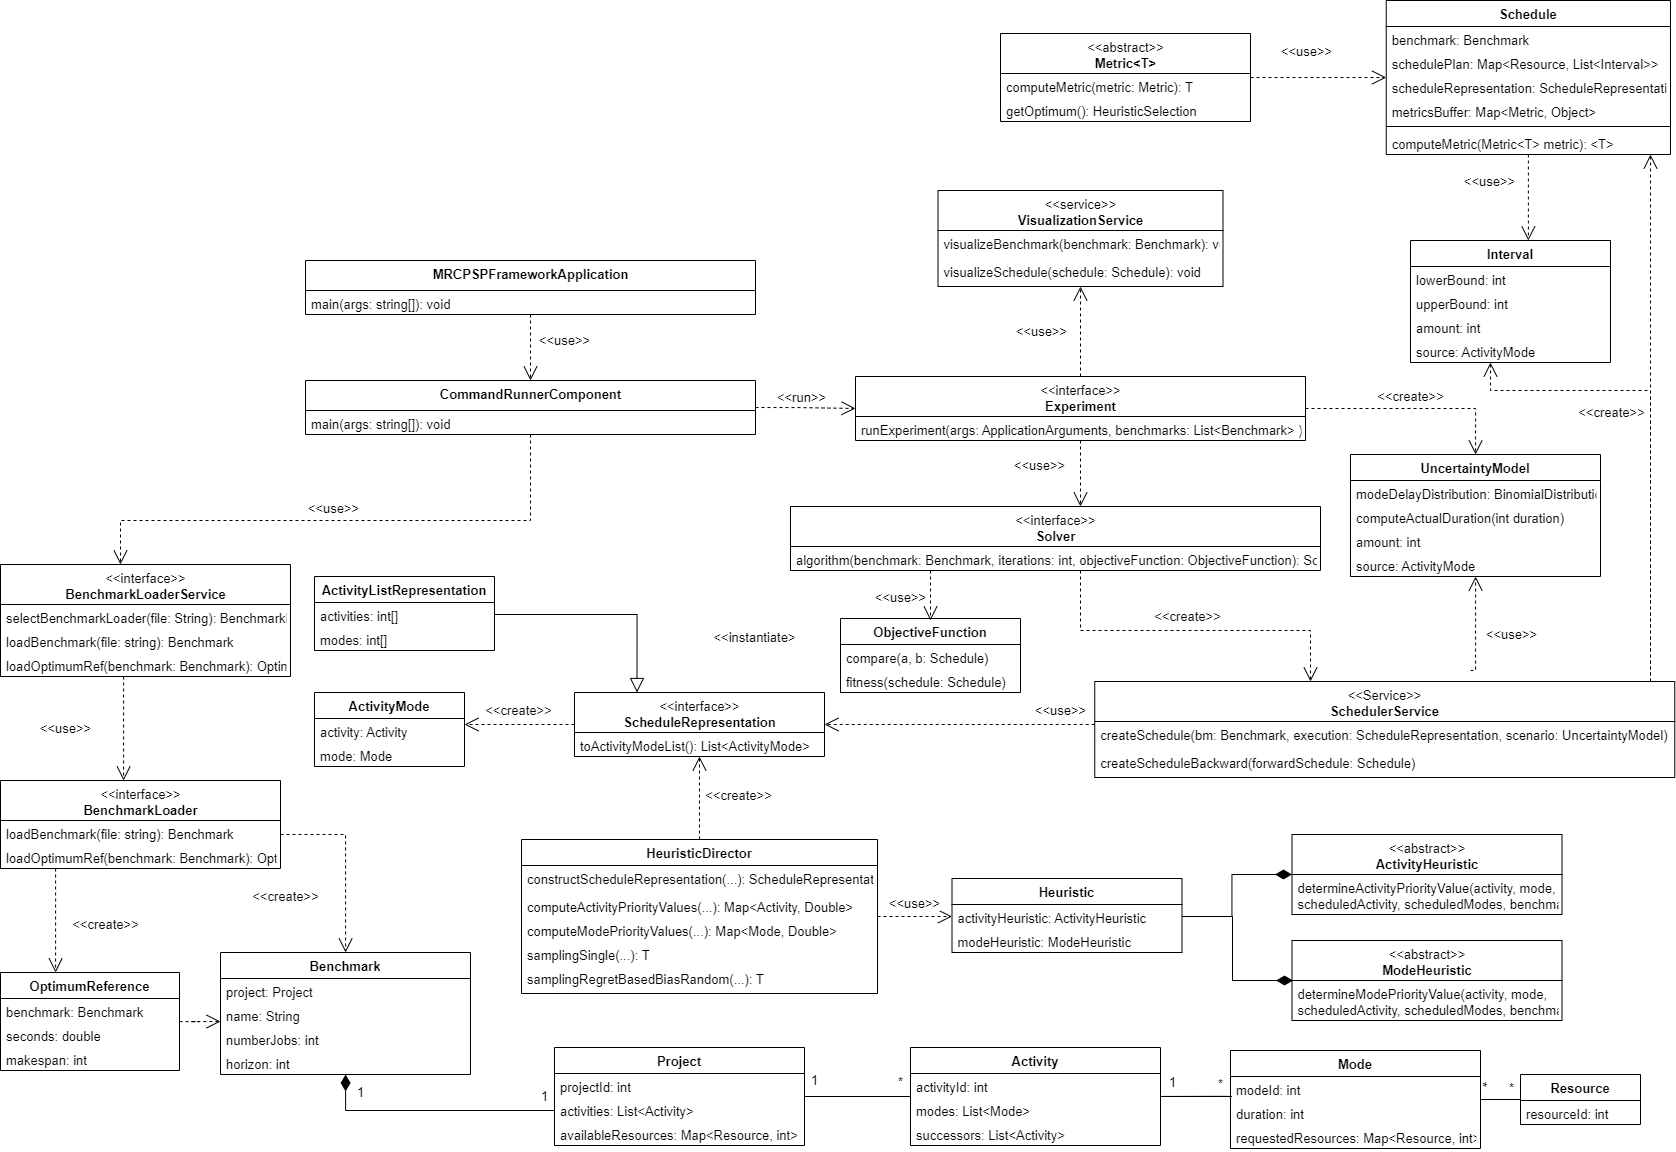
\includegraphics[angle=90,height=0.90\textheight]{assets/img/04_Umsetzung/Klassendiagramm_Minimized.drawio.png}
    }
    \caption{Zusammengefasstes UML-Klassendiagramm des MRCPSP-Framework} 
    \label{img:mrcpsp_framework_klassendiagramm}
    \source{Eigene Darstellung}
\end{figure}

Durch die Implementierung entstand das zusammengefasste UML-Klassendia-gramm aus Abbildung \ref{img:mrcpsp_framework_klassendiagramm}, welches aufgrund der Komplexität keine Generalisierungen von abstrakten Klassen und Interfaces berücksichtigt. Im Verlauf des Kapitels werden einzelne UML-Klassendiagramme zur Erläuterung der Umsetzung eingesetzt und erläutert, welche diese Generalisierungen aufführt. 

\newpage